\documentclass[11pt,a4paper]{jsarticle}
\usepackage[dvipdfmx]{graphicx}
\usepackage{graphicx}
\usepackage[top=20truemm,bottom=20truemm,left=25truemm,right=25truemm]{geometry}
\usepackage{comment}


\title{Si基板上のスズ}
\author{平松信義}
\date{\today}
\begin{document}
\maketitle

まずαスズ結晶における銅の特性X線(K$\alpha$1:$\lambda$=1.5405\AA; K$\alpha$2:$\lambda$=1.5443\AA)の回折を考える。
先行研究\cite{gray}からαスズ(粉末)を格子定数$a=6.4892\AA$のダイアモンド構造とすると、スズの結晶面(111)の格子面間隔は$d=a/\sqrt{1^2+1^2+1^2}=3.7465\AA$であり、結晶面(111)で回折されたピークは2$\theta$=23.730$^\circ$(K$\alpha$1)と2$\theta$=23.788$^\circ$(K$\alpha$2)に現れる(図1赤色左端のピーク)。ここでBraggの回折公式$2dsin\theta=n\lambda$を用いた。

図1のSi基板上のスズメッキ試料(灰色と黒色)でαスズに起因する回折ピークは2$\theta$=22.4$^\circ$に現れており、Braggの回折公式より格子面間隔$d=3.96\AA$に対応する。これを粉末αスズの結晶面(111)の格子面間隔$d=3.7465\AA$と比較すると5.8\%大きく、Si基板上のαスズが数\%歪んでいることを示唆する。

一方βスズの歪みは0.5\%程度以下である。図1のSi基板を研磨後メッキした試料(灰色)はβスズに起因する回折ピークが現れている(2$\theta$=30.7$^\circ$; 32.0$^\circ$)が、粉末βスズのピーク(2$\theta$=30.64$^\circ$, 30.72$^\circ$; 32.03$^\circ$, 32.10$^\circ$)\cite{white}と比較すると、その差は高々$\Delta(2\theta)=0.2^\circ$程度だった。これから格子面間隔の差(歪み)を計算すると$\frac{\Delta d}{d}=cot\theta \Delta\theta= 0.003$だった。

\begin{figure}[!h]
    \begin{center}
   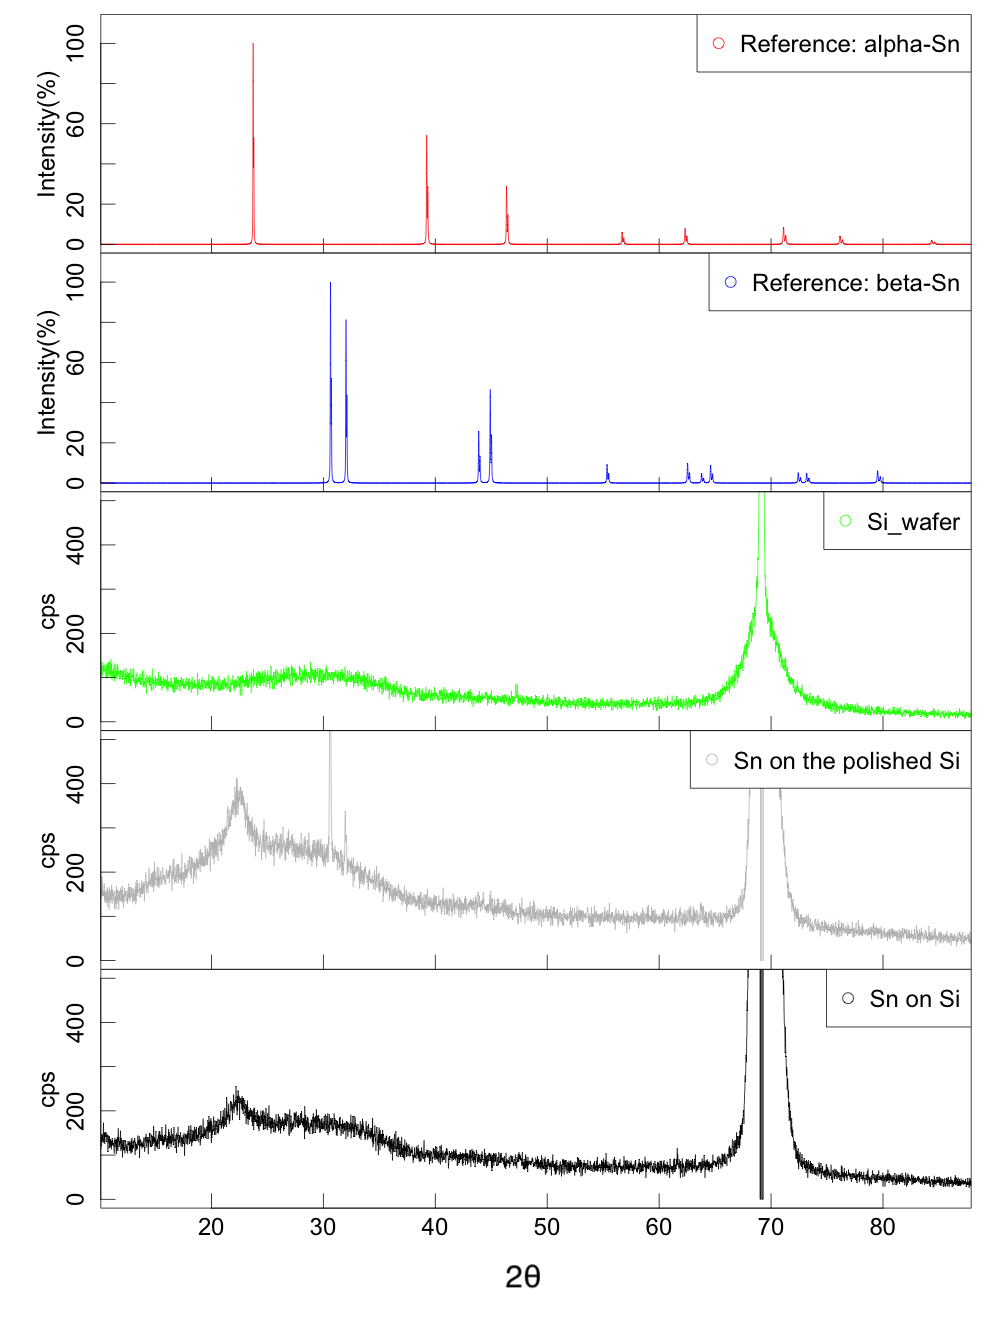
\includegraphics[width=0.6\hsize]{Sn_on_Si.eps}
  \end{center}
  \caption{Si基板上のスズのX線回折強度}
  \label{fig:Sn_on_Si}
\end{figure}



\begin{thebibliography}{9}
\bibitem{gray} J. Thewlis, and A. R. Davey,  Thermal Expansion of Grey Tin, Nature 174, 1011 (1954)  
\bibitem{white}M. Wolcyrz , R.  Kubiak, and S. Maciejewski, X‐ray investigation of thermal expansion and atomic thermal vibrations of tin, indium, and their alloys. Phys. Stat. Sol. (b) 107,  245 (1981)
\end{thebibliography}

\end{document}